% !TEX root = ../Dissertation.tex
%===================================================================================================

\chapter{Data Collection}




\section{B cells are developing in the NOD thymus}

The reason for B cells being present in the thymus is unknown. 
The potential mechanisms, as outlined in \toref{somewhere in background} are B cells developing from progenitors within the thymus or B cells are being released prematurely from the bone marrow and migrating to the thymus where they continue and complete their development.
Data to date suggests that B cells are developing in the thymus due to the fact pro and pre B cells can be seen there. 
However, there are also other methods for investigating potential intrathymic B cell development.
This project focuses on the following areas of investigation:

\begin{enumerate}
\item Utilisation of flow cytometry to look for pro and pre B cells in the thymus of NOD mice and to see how the state of the NOD thymus compares with other control mice.\toref{relevant subsection}

\item Utilisation of flow cytometry to look for very early progenitors at the initial stages of B cell commitment within the thymus. 
This required the use of magnetic-activated cell sorting (MACS) to deplete thymi of mature cells to reveal the smaller progenitor populations. 
The presence of early B cell progenitors in the thymus could then be compared between NOD mice and controls. \toref{relevant subsection}

\item Utilisation of polymerase chain reaction to investigate the presence of transcription factors and genes driving B cell development in the  thymus. \toref{relevant subsection}
\end{enumerate}

Each will be discussed in the relevant sections below.

\subsection{There are pro and pre B cells present in the NOD thymus}


As mentioned previously, following commitment to the B cell lineage, B cells develop through different developmental stages.
The first is the CD19+CD43+IgM- pro B cell stage.
Following this, IgM heavy chain rearrangement begins and the developing B cells produce an IgM heavy chain. 
They can then progress to the CD19+CD43-IgM- pre B cell stage.
Finally, in the bone marrow, B cells produce a fully functioning B cell receptor (IgM) and are then a CD19+CD43-IgM+ immature B cell.
These immature B cells then move to the spleen to finish their development and become mature B cells.


\subsection{Developing B cells in the thymus express RAG}

Interestingly, of the CD19+ cells present in the NOD and B6 mice, although the majority are mature IgM+ B cells, there are also populations of developing B cells at the pro and pre B cell stages.
This gives the impression that B cells are developing within the thymus rather than migrating there and warrants further investigation. \fig{Add figure showing pro and pre B cells}

To try and identify whether or not pro and pre B cells are developing within the thymus rather than migrating there, the expression of RAG in these developing B cells was investigated.
To do this, a NOD-RAG-GFP reporter mouse was used as this mouse produces GFP when RAG is being expressed.
GFP shows up on flow cytometry therefore it is a useful tool for investigating B cell development.
RAG expression is crucial during B cell development as it allows the rearrangement of the IgM heavy chain and thus allows the progression from pro to pre B cell stage.

Thymi and bone marrow from NOD-RAG-GFP mice of 4, 7 and 11 weeks of age were used for flow cytometry to look for the present of RAG+CD19+ cells.
Positive RAG expression in CD19+IgM- cells would indicate active development.
As shown in \fig{add figure showing RAG high, low, neg in CD19+ cells in thymus}

The intensity of the RAG signal is important for determining the liklihood of active development.
Since GFP is transcribed at the same time as RAG, it initially has a very high intensity.
However, because GFP is a protein it takes a while to degrade and has a half life of ~54hrs.
This means that only the CD19+RAGhigh population can be taken as actively expressing RAG and therefore GFP.
GFPlow cells will have deactivated RAG and therefore the GFP signal will be decaying.
Setting the gates for RAG\textsuperscript{high} and RAG\textsuperscript{low} populations was done by looking at the RAG levels in developing B cells in the bone marrow.

As shown by the \fig{figure of RAG high, low etc} and graph \fig{graph showing RAG high low neg over different ages}, the frequencies of CD19+RAG\textsuperscript{high} \todo{look at how frequencies of CD19+RAG+ cells change with age}. This suggests that... \todo{explanation?}





\fig{Pro and Pre cells present in the NOD thymus. Show a plot of IgM vs CD43 and label which quadrants are pro and pre.}
\fig{\%s of pro and pre in different ages and strains}
\fig{ratios of pro:pre in thymus vs BM. any difference in different strains?}



\subsection{B cell development is dependent on the presence of a mature B cell}

Following on from this finding, B cell KO NOD mice thymi were also investigated.
In these mice, as stated in \toref{wherever I talked about KO mice}, these mice are unable to rearrange their IgM heavy chain and therefore cannot progress beyond the pro B cell stage. 
In the bone marrow of these mice, a population of pro B cells is seen, but there are no pre B cells and no IgM+ cells.
It was therefore expected that in their thymus there would also be a population of pro B cells, similar to that seen in the NOD WT mice. 
However, this does not appear to be the case.
As shown in \fig{add figure showing decreased pro B cells in KO thymi}, it appears that the frequency of pro B cells in the thymus is consistently decreased in B cell KO mice compared to NOD WT mice.
Interestingly, the frequency of IgM-CD43+CD19+ cells in the thymi of KO mice is lower than the frequency seen in the B6 control mouse. 
This gives the impression that a mature B cell is important for allowing the enhancement of pro B cells in the thymus.
Moreover, the need for a mature B cell is more important to increase thymic pro B cells than whatever mechanism is present in the NOD mouse strain that increases the intrathymic pro B cell presence.
The investigation was carried out in a blind trial so that the strains of mice were not known during analysis in order to avoid bias in the results.

\fig{Difference in pro B cells in WT, KO and B6.}
\todo{suggest a transfer experiment/chimera formation to test whether transfer of mature B cells into a KO mouse increases the population of pro B cells in the KO thymus}



\subsection{Early B cell progenitors are present in the NOD thymus}

\subsubsection{Introduction to progenitor work}

Given the discrepency between the NOD mouse and the B6 control mouse in terms of B cell numbers in the thymus, it was decided that investigation into the presence of B cell progenitors in the thymus would be beneficial.
As mentioned in , the progenitor populations giving rise to T and B cells is controversial and there does not appear to be a proven pathway for the development of either.
This leaves a number of questions relating to how these populations can be investigated.
However, literature to date suggests developmental pathways for each and it is this information which has driven the investigation into thymic B cell progenitors.

Of particular interest in this project, information relating to the earliest B cell committed progenitor was sought.
There is much research pertaining to B cell development in the bone marrow and the factors driving the development but it remains a highly complex area.
The matter was complicated further in this project due to the fact B cell development was being investigated in the thymus rather than the bone marrow.
This means that research into this area was based on previous research in the bone marrow and how well B cell development in the bone marrow is mirrored by potential development in the thymus remains unknown.

 However, assuming that B cell development in the thymus was to follow the same pathway as that seen in the bone marrow, the pattern of development should follow the course shown below.

 
\todo{Diagram of B cell development. Show HSCs through MPPs to ALPs/BLPs etc}


 It is not totally clear as to what phenotype the earliest B cell committed progenitor has. 
 However, there is evidence that expression of Ly6D correlates with almost total B cell restriction \toref{Inlay}.
 With this is mind, it was possible to use flow cytometry with an appropriate mix of antibodies to investigate the presence of Ly6D+ progenitors in both the thymus and bone marrow of NOD mouse.
However, Ly6D alone is not sufficient to indicate B cell restriction. 
It is also seen that developing T cells express Ly6D and therefore other markers are required to show which progenitors are likely to B cell restricted rather than T cell restricted.
The markers used alongside Ly6D therefore were Sca-1, c-kit, IL-7Ra and Flt3. 
The reasons for using each of these antibodies are outlined below.
\begin{itemize}
\item Sca-1 - 
\item c-kit - This is expressed at greater levels on T cells compared to B cells therefore in gating of data looking for B cell progenitors, care was taken to not include c-kit high cells as these are likely to B of T cell lineage \toref{Find a reference for this} 
\item IL-7Ra - 
\item Flt3 - The expression of Flt3 on progenitors denotes the retention of B and T cell lineage potential. Therefore, when looking for progenitors that have the potenital to become either a T or B cell, the expression of Flt3 shows that it is not yet committed to the T cell lineage.
\toref{Karsunky2008}
\item Ly6D - \toref{Inlay, Mansson, Zhang2013}
\end{itemize}




The thymus is the site of T cell development and education.
The progenitors for T cells, however, are not totally understood. 
There is belief that T cells originate from CLPs which have migrated from the bone marrow to the thymus where they receive the correct signals which cause them to differentiate into T cells
\subsection{Magnetic-assisted cell sorting optimisation}

Due to the small size of progenitor populations in comparison to mature cell populations in the thymus, it was first necessary to deplete the thymus of the majority of mature cells before looking for progenitors.
For depletion, magnetic-activated cell sorting (MACS) was used.
There are many different kits available and the decision on which to use for the experiments was taken after investigating the efficiency and yield from Miltenyi beads and columnms, and Qiagen anti-rat beads \todo{name of Qiagen beads}

Firstly, Miltenyi columns and lineage depletion beads were tested to assess their efficiency. 
\fig{add figure showing efficiency of beads/columns here}.
To start with, only one round of depletion was carried out which gave an efficiency of \todo{look at efficiencies}.
This efficiency was improved to \todo{add efficiency of 2 rounds} when two rounds of depletion were carried out \fig{2 round miltenyi lineage depletion}. 
\begin{figure}
	\begin{subfigure}{\textwidth}
	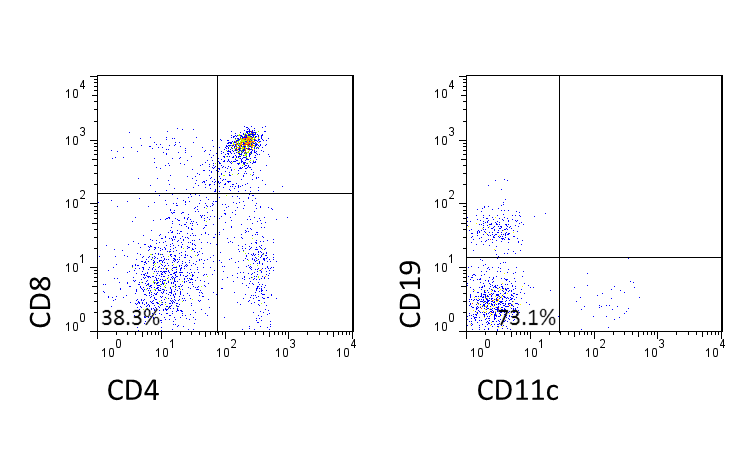
\includegraphics[width=\textwidth]{Figures/1rounddepletion.png}
	\caption{One round of depletion using Miltenyi lineage depletion beads and columns}
	\end{subfigure}
	\hfill
	\begin{subfigure}{\textwidth}
	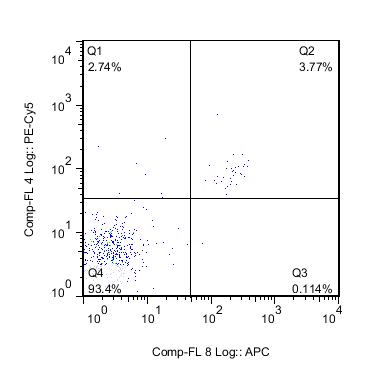
\includegraphics[width=0.3\textwidth]{Figures/2rounddepletion.png}
	\caption{Two rounds of depletion using Miltenyi lineage depletion beads and columns}
	\label{subfig:2miltenyi}
	\end{subfigure}
	\hfill
	\begin{subfigure}{\textwidth}
	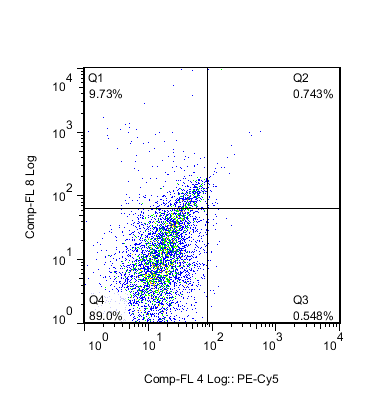
\includegraphics[width=0.3\textwidth] {Figures/Qiagenbeads.png}
	\caption{Qiagen Beads}
	\label{subfig:Qiagen}
	\end{subfigure}
	
\caption{Figure showing the different methods of depletion. Qiagen beads in shows that 89\% percent of cells are CD4-CD8-}
\end{figure}
However, while this method gave a very pure sample with very few mature cells remaining, the yield was not very good.

Since the point of the depletion was just to reduce the quantity of mature cells so that the progenitor populations could be seen by flow cytometry, it was more important for the experiment that there was a lot of cells to interrogate rather than them being very pure.
Therefore, Qiagen beads were tried and as shown, \fig{figure of Qiagen depletion}, while the purity was not as good as the Miltenyi beads \todo{efficiency of Qiagen beads}, the yield was much improved.
This was a better balance for the experiment, therefore, Qiagen beads were used.
\todo{insert a table showing the efficiencies of each depletion method}

\todo{analyse results comparing NOD/KO/B6 data to see if the presence of BLPs is normal in NOD}
Once the method of lineage depletion was decided on, it was then possible to move forward to investigating the early progenitor populations in NOD, NOD KO and B6 thymi.
BLP presence was of particular interest as differences in populations between strains of mice could suggest whether the increase in B cells in the NOD thymus was as a result of processes before or after this point.
BLPs are thought to be the first cell committed to the B cell lineage therefore if the populations of these cells are different, it could suggest abnormalities in factors driving B cell commitment.

\fig{Gating system: LCs, SCs, sca int, kit int, IL-7Ra+Flt3+, Ly6D (+ in BLPs/pre-pro, - in ALPs)}
\fig{?\% of BLPs, ALPs and MPPs in each strain}
\fig{?Ratios of BLP:ALP in BM and thymus}


\subsection{T cell development looks normal/abnormal in NOD mouse compared to control}
\fig{CD4 v CD8, CD44 v CD25}
\fig{\%s of CD4, CD8, DN, DP in each strain. How does NOD WT compare to NOD KO? How does B6 compare to FVB? How does NOD compare to controls?}
\todo{analyse data to see whether it is normal or abnormal. This is a good control to give an indication of the overall condition of the thymus, preferably over time to see how it changes as mouse ages with normal physiological atrophy of the thymus}

\subsection{The NOD thymus contains B cell development transcription factors}

If B cells are developing within the thymus, this begs the question as to whether the NOD thymus is providing an environment more conducive to B cell development compared to nondiabetic controls. 
To invesitgate this, primers were designed that were specific for B cell development factors such as E2A, EBF, Pax5, VPreB and CXCL12.
\todo{look in Hagman2006, Welinder2011, Mansson2008, Cobaleda2007, Radtke2013, Riley2013, Tokoyoda2004 for TF info}.

To date, only regular PCR has been carried out to compare whether or not B cell development transcription factors are present in the NOD bone marrow and thymus.
Since normal B cell development occurs in the bone marrow, these transcription factors would be expected there and indeed they were seen there, as shown in \fig{TF gels}. 
Interestingly, all the genes, besides CXCL12, were also present in the NOD thymus too.
This indicates that the thymic environment may also be allowing B cell development.
The lack of CXCL12 in the thymus is not a surprising result as it is a cytokine responsible for holding developing B cells in the bone marrow niche and therefore, may be more bone marrow specific rather than B cell specific.



\fig{regular PCR looking for transcription factors (VPreB, Pax5, EBF, E2A, CXCL12)}

\todo{qPCR of Pax5, Notch, EBF etc}
\fig{qPCR results}

\subsection{Conclusion}

Data to date has so far given evidence that B cells are developing intrathymically in the NOD mouse.
This is shown by pro and pre B cells being present suggesting that developing B cells are present in the thymus.
Further to this, some of these cells show evidence of active RAG expression, indicating that they are actively developing within the thymus rather than having migrated there following premature release from the bone marrow.

There is also evidence to suggest that B lineage committed early progenitors, such as BLPs, are present within the NOD thymus. 
This also gives the impression that B cells are developing from progenitors within the thymus as these are believed to be the progenitors that pro B cells are derived from.
\todo{Add conclusion on differences in frequencies of BLPs in NOD/B6/KO etc to see if any difference}

Finally, it appears that the NOD thymus may be providing factors that are allowing, if not driving, B cell development.
However, it remains to be seen whether this is a normal finding in nondiabetic controls also.
It would also be useful to carry out quantitative PCR of B cell development factors to see the relative levels between the thymus and bone marrow and across strains of mice.
This could suggest whether or not it may be a thymic abnormality in the NOD mouse which is providing a particularly good environment for B cell development compared to other strains of mice.

\section{Some RAG+ cells in the thymus express B and T cell markers}
During analysis of data from previous experiments, it was noted that a large proportion of RAG+CD19+ cells in the NOD thymus, were also CD4+CD8+.
This was of interest and was therefore investigated further.

\subsection{A large proportion of RAG+CD19+ cells in the NOD thymus express CD4 and CD8}

\cref{fig:RAGCD19CD4CD8pos}

Whilst looking for RAG+CD19+ developing B cells in the NOD thymus, analysis of these cells showed that they were also expressing CD4 and CD8. 
This suggests that there are cells developing in the thymus, shown by the expression of RAG, that are not yet lineage committed and are expressing markers of both T and B cells.
It could suggest that there is a mechanism by which T cells are becoming B cells or vice versa.
The gating pattern used to look for these cells in the thymus and bone marrow of NOD WT and NOD KO is shown in \cref{fig:RAGposDP}.
However, it was not known if this is normal during B cell development, therefore the bone marrow was used as a comparison to see if these cells existed there too, where B cells develop normally.
Interestingly, there were no RAG+CD19+CD4+CD8+ cells seen in the bone marrow at all. 
The comparison between a representative 4 week old NOD thymus and bone marrow is shown in \cref{subfig:BMvsThyRAGCD19DP}.
The presence of these RAG+CD19+CD4+CD8+ cells in the thymus was consistent and seen in 4 week and 7 week old NOD thymi with group sizes of 4 or 5 mice in each age group. 
The lack of these cells in the bone marrow suggests that they may be thymus-specific.
However, whether or not the presence of these cells has any relation to the increased population of thymic B cells seen in the NOD mouse remains to be determined.
One way of investigating this is to use non diabetic, control B6 mice.


These cells are present in NOD mice at both 4 and 7 weeks of age and it was therefore investigated whether or not there was a significant difference in the percentages of these cells between the two age groups. 
The bone marrow is also included in the figure as a comparison.
The results of this comparison are shown in \fig{add a graph showing how the ages affect the presence of RAG+CD19+DP cells in the thymus and bone marrow}
\todo{add some data/graph/statistics to show significance, whether there is a difference between the ages etc}


\begin{figure}	
	\begin{subfigure}{\textwidth}
		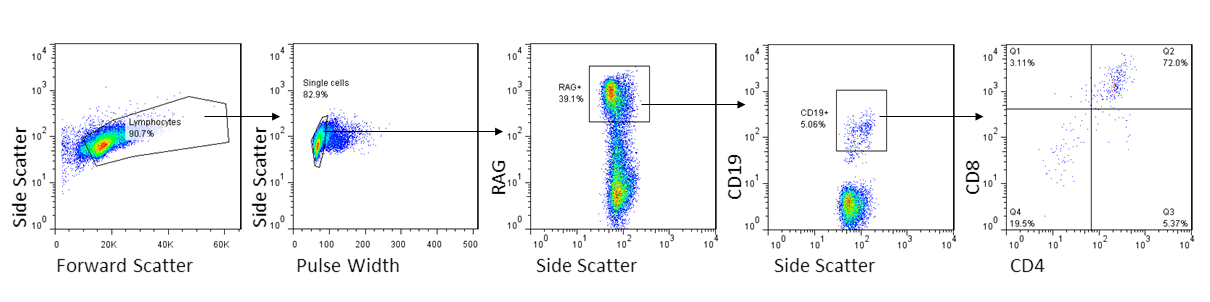
\includegraphics[width=\textwidth] {Figures/CD19+RAG+DPgating.png}
		\caption{Figure showing the gating pattern when looking for RAG+CD19+CD4+CD8+ cells in a NOD thymus.}
		\label{fig:RAGposDP}
	\end{subfigure}
	\begin{subfigure}{\textwidth}
	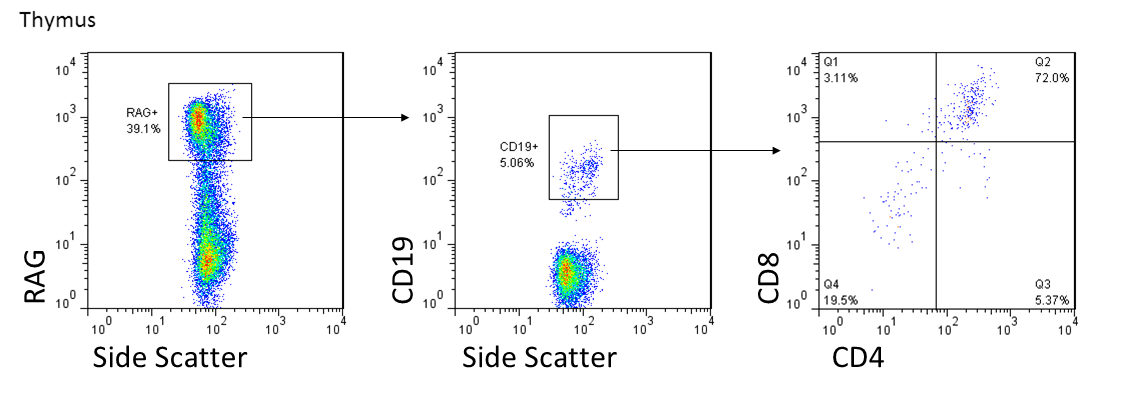
\includegraphics[width=0.5\textwidth]{Figures/Thymus1RAGCD19DP.png}
	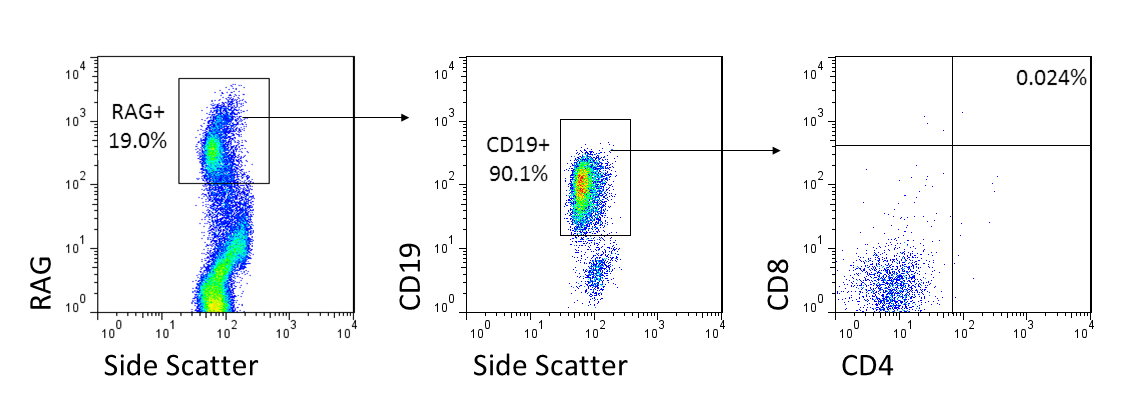
\includegraphics[width=0.5\textwidth]{Figures/BM1RAGCD19DP.png}
	\caption{Representative plots to show the difference in presence of CD19+RAG+CD4+CD8+ cells in the NOD thymus and bone marrow}
	\label{subfig:BMvsThyRAGCD19DP}
	\end{subfigure}
\caption{This figure is about RAG+CD19+CD4+CD8+ cells in the NOD thymus of 4 and 7 week old NOD mice}
\label{fig:RAGCD19CD4CD8pos}
\end{figure}



\subsection{RAG+IgM+TcRb+ cell presence in the NOD thymus}
It was then also investigated as to whether the developing cells expressing RAG, CD19, CD4 and CD8 could potentially progress to being RAG+CD19+IgM+TcR+ and therefore express mature T and B cell markers.
Data for this is shown in figure \cref{fig:RAGIgMTcRpos}

\begin{figure}
	\begin{subfigure}{\textwidth}
	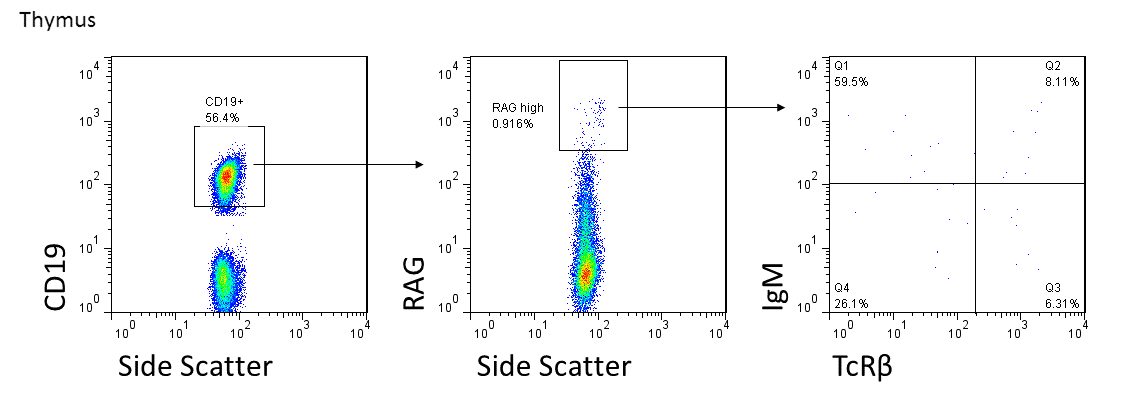
\includegraphics[width=0.5\textwidth]{Figures/Thy3RAGIgMTcR.png}
	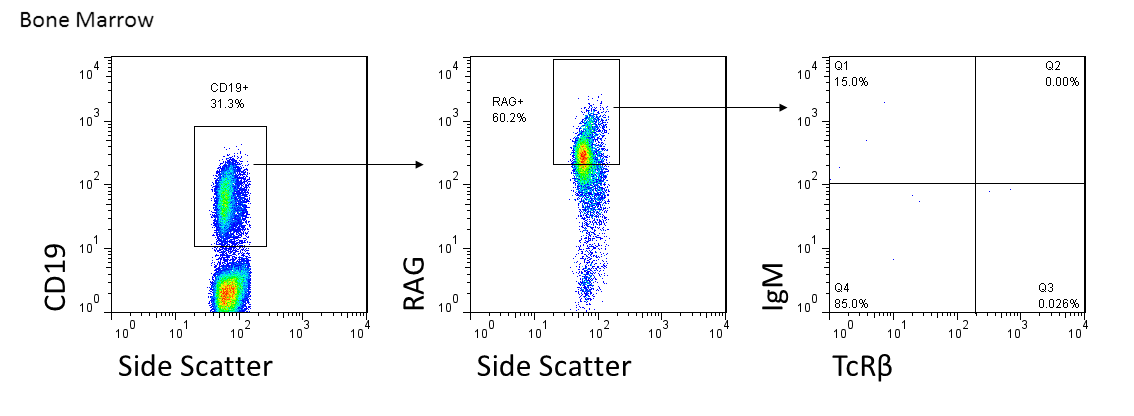
\includegraphics[width=0.5\textwidth]{Figures/BMRAGIgMTcR.png}
	\caption{Representative thymus and bone marrow analysis looking for RAG+IgM+TcR+ cells}
	\label{subfig:BMvThyRAGIgMTcR}
	\end{subfigure}
\caption{This figure is about RAG+IgM+TcR+ cells in the NOD BM and thymus. 5 thymi and one bone marrow were analysed from 5 11week old NOD mice.}
\label{fig:RAGIgMTcRpos}
\end{figure}

\subsection{IgM+TcRb+ cell presence}
Following on from this, the aim was to see if these cells develop further and begin to express both a T and B cell receptor, in this case, TcRb and IgM.
To do this, flow cytometry was carried out on thymic samples from NOD, NOD KO and B6 mice using antibodies specific to TcRb and IgM.
This time, the spleen was also investigated alongside the thymus and bone marrow to provide another comparison and to widen the search for IgM+TcR+ cells.
Mice of various different ages were investigated and the results are shown in \fig{figure showing TcR+IgM+ cells (or not!)} .
Isotype controls were also carried out to help with determining whether cells were expressing TcR or IgM or not.
The data from the isotype controls in shown in \fig{isotype controls}.
\todo{include isotype control data}


\subsection{Conclusion}
Following on from the flow cytometric data acquired so far relating to the presence of IgM+TcR+ cells in the NOD thymus, it appears that these cells do not exist. 
It may be that the RAG+CD19+CD4+CD8+ cells seen in the thymus are early cells developing in the thymus which are not yet totally committed to one lineage and are expressing markers of multiple lineages, hence the T and B cell markers.
However, it would be beneficial to carry out investigation at the protein level, for example, Western Blotting, in order to see if more mature cells are expressing T and B cell receptors.




\section{Potential contribution of thymic B cells to T1D}

\subsection{Pilot study to track movement/homing of thymic B cells on transfer into recipient mice}
\todo{where B cells traffic to could give indication of their role in T1D. Also, use of GFP as  a marker. However, numbers were very small so analysis difficult. Needs to be done again in the future. Comment on whether it may be possible and what would need to change to make it work. Also decide on which transfer experiment I am referring to.. NOD to KO or GFP to NOD...}
In order to look at the potential impact that thymic B cells may be having on the pathogenesis of T1D, a pilot study looking at the migration of donor thymic B cells following intravenous injection into recipient mice was set up. 
At time points of 7 and 11 days post injection, recipient mice were sacrificed and their thymus, spleen, bone marrow, pancreas, pancreatic lymph node and lateral axillary lymph node were all analysed by flow cytometry.
The tissues to analyse were chosen for the following reasons:
\begin{itemize}
\item Thymus - The thymus is the tissue where the donor cells were taken therefore it was included in analysis to see if the donor cells would migrate back to the thymus in the recipient cells.
This would give the impression that thymic B cells have specific properties which allow them to traffic back to the thymus.
For example, they may have specific cytokine sensitivity which results in being able to home back to the thymus following transfer.
\item Spleen - The spleen was included for analysis as this is the normal site of B cell maturation.
Therefore it was of interest to see if thymic derived donor cells would move here like conventional B cells do to finish development.
\item Bone marrow - The bone marrow is the normal site of B cell development and therefore was included to see if the developing donor B cells would preferentially to here to develop in the same way as conventional B cells
\item Pancreas - The pancreas contains the Islets of Langerhans which are destroyed in T1D through T and B cell mediated attack.
Pancreatic tissue was therefore analysed to see if thymic B cells migrate to here preferentially upon transfer into recipient mice.
If so, it may indicate that thymic B cells could have a direct role in the pathogenesis of the disease.
\item Pancreatic lymph node - The PLN is where antigen-presenting cells move to from the pancreas in order to activate T cells.
In T1D, APCs move from the pancreatic islets to the PLN carrying islet antigens and therefore the PLN is in an inflammatory state.
This tissue was therefore included to look at the status of the lymph node to compare it to the control axillary lymph node.
\item Lateral axillary lymph node - This tissue was analysed as a control to compare to the PLN.
Whereas the PLN should be inflamed in T1D, the lateral axillary lymph node should not and can therefore show that any inflammation in the PLN is localised and is not as a result of inflammation throughout the body.
\end{itemize}

\todo{Questions to ask of data: 1) Where do B cells go? 2)Do the B cells survive? 3) Is GFP a good tracker? 4) Do you get B cells in the CD19- recipients? 5) DO CD19+ cells increase in KOs after transfer? Can't tell as can't differentiate between donor and recipient) 6) Is there new GFP activation after transfer?}

\subsection{Autoantibody production}
\todo{analyse the FACS of the stroma to look at the purity of stromal cells that will have been put on the microscope slide}
\fig{Representative FACS showing stromal purity}
\fig{Pictures of histology showing serum treated and control PBS treated slides}

\subsection{Conclusion}


